
%\usepackage{pgfplots}
%\usepackage[ISO]{diffcoeff}
%\diffdef{}{ op-symbol=\mathsf{d} }
%
%\pgfplotsset{compat=1.18}
%
\chapter{Special Relativity}

%  This is the \emph{extended version}\footnote{Think of this as the
%    ``director's cut'' that will never be shown in a theatre, or a classroom
%    in this case} of the slides presented in Class 14. It is intended for
%  students who are interested in more details than presented in class. It also
%  includes some calculus that is definitely not required for the course. To
%  present all the information  will require about 3 classes of lecturing, which
%  is not practical at this level.
%
%
%y
%
%\section{What Everyone Thinks They Know}
%  
%  {\fontsize{50}{60}
%    \begin{displaymath}
%      \boxed{E=mc^2}
%    \end{displaymath}
%  }
%  
%  \vspace{.2in}When we think of relativity, most people think of \emph{this}
%  equation\footnote{A certain physics teacher at Meritus Academy had this
%    equation printed on a t-shirt during their teenage years, much to the
%    delight of school bullies.}, but what does it actually mean? And more
%  importantly, how did it come about?
%
%
%\section{Frame of Reference}
%  A \textbf{frame of reference}\footnote{Or \textbf{reference frame}, or just
%    \textbf{frame}.} is the \emph{coordinate system} in which physical
%  measurements are made. In \emph{classical} mechanics, a frame of reference is
%  \begin{itemize}
%  \item the $x$- $y$- and $z$-axes in the Cartesian coordinate system
%  \end{itemize}
%  \vspace{.2in}However, it may be more useful to think of the frame of
%  reference as a ``hypothetical mobile laboratory'' an observer uses to make
%  physical measurements (e.g.\ mass, lengths, time). At a minimum, it includes:
%  \begin{itemize}
%  \item A set of rulers (i.e.\ a coordinate system) to measure lengths
%  \item A clock to measure the passage of time
%    %\item A scale to compare forces
%    %\item A balance to measure masses
%  \end{itemize}
%
%
%
%
%\section{Review: Frame of Reference}
%  \begin{itemize}
%  \item We assume that the ``hypothetical laboratory'' is \emph{perfect}
%    \begin{itemize}
%    \item The hypothetical ``instruments'' have zero errors
%    \item There are perfect instruments to measure anything you want
%    \end{itemize}
%  \item What matters is the \emph{motion} (at rest, uniform motion, acceleration
%    etc) of your laboratory, and how it affects the measurement that you make
%  \item ``From the point of view of\ldots''
%  \end{itemize}
%
%
%
%
%\section{Newtonian (Classical) Relativity}
When we studied \emph{classical physics}\footnote{Also known as
\emph{Newtonian} physics because of Newton's contribution}, we made some
untested assumptions:
\begin{itemize}
\item\textbf{Absolute space:} \SI1{\metre} is \SI1{\metre} no matter where
  you are and how you are moving
\item\textbf{Absolute time:} \SI1{\second} is \SI1{\second} no matter where
  you are and how you are moving
\end{itemize}
Under these assumptions, measurements of space and time are \emph{independent}
of motion of the observer. It also means that:
\begin{itemize}
\item\emph{All} velocities are relative to the frame of reference of the
  observer
\item There is no such thing as \emph{absolute motion} or \emph{absolute rest}
\item Motions of different frames of reference are related by the
  \textbf{Galilean velocity addition rule}:
  \begin{equation*}
    \vec v_{AC}=\vec v_{AB}+\vec v_{BC}
  \end{equation*}
\end{itemize}




%\section{Inertial Frame of Reference}
%  An \textbf{inertial frame of reference}\footnote{It is also known as a
%    \textbf{rest frame} for obvious reasons} is one that is moving in uniform
%  motion (i.e.\ constant velocity, zero acceleration)
%  \begin{itemize}
%  \item In an inertial frame, the laws of motion are valid
%  \item An observer may consider any inertial frame to be at
%    rest\footnote{i.e.\ stationary}
%  \end{itemize}
%  
%  \vspace{.15in}The concept of inertial frame of reference originated from
%  Galileo's time, a few decades before Newton, and is incorporated into how
%  physical laws are constructed:
%  \begin{center}
%    \fcolorbox{black}{yellow!10}{
%      \begin{minipage}{.85\linewidth}
%        \textbf{The Principle of Relativity:} All laws of motion are equal in
%        all inertial frames of reference.
%      \end{minipage}
%    }
%  \end{center}
%
%
%
%
%\section{Example: Inertial Frame of Reference}
%  \begin{itemize}
%  \item Observer A is ``moving'' uniformly with the skateboard
%    \begin{itemize}
%    \item It is valid for A to think that he is at rest, but B (and the rest of
%      the world) is moving
%    \end{itemize}
%  \item Observer B is standing on the side of the road
%    \begin{itemize}
%    \item It is valid for B to think that he is at rest, but A (and his
%      skateboard) is moving
%    \end{itemize}
%  \item A \& B observe different motion, but they agree on the \emph{physical
%    law} that governs that motion
%  \end{itemize}
%  \begin{center}
%    \vspace{-.1in}
%    \pic{.65}{graphics/57}
%  \end{center}
%
%
%
%
%
%
%%\section{New Physics: Maxwell's Equations}
%%  
%%    \centering
%%    \pic{1.2}{graphics/PORTRAIT-James-Clerk-Maxwell}\\
%%    James Maxwell
%%    
%%    \begin{itemize}
%%    \item For centuries, experimental results would always agree with this
%%      ``Newtonian'' framework\ldots
%%    \item By 1870s, instruments became accurate enough to measure behaviours
%%      that were slightly different from prediction
%%    \item \textbf{Maxwell's equations} in 1861 and 1862 are classical laws of
%%      electrodynamics that explains the relationship between
%%      \begin{itemize}
%%      \item Electricity
%%      \item Electric Circuits
%%      \item Magnetism
%%      \item Optics
%%      \end{itemize}
%%    \end{itemize}
%%  
%%
%
%
%
\section{Maxwell's Equations}
\textbf{Maxwell's equations} relate any disturbances in the electric and
magnetic fields to the formation of a travelling \textbf{electromagnetic
  wave}\footnote{Also known as the \textbf{EM wave}, or
\textbf{EM radiation}}:
%
%  \vspace{-.2in}{\large
%    \begin{align*}
%      \nabla\cdot\vec E &=\frac\rho{\varepsilon_0}\\
%      \nabla\cdot\vec B &= 0\\
%      \nabla\times\vec E &=-\frac{\partial\vec B}{\partial t}\\
%      \nabla\times\vec B &=-\mu_0\vec J+
%      \mu_0\varepsilon_0\frac{\partial\vec E}{\partial t}
%    \end{align*}
%  }

In a vacuum, Maxwell's equations predict that all EM waves travel with a speed
($c$) defined by the permeability of free space ($\mu_0$) and permittivity of
free space ($\varepsilon_0$):
\begin{equation}
  \boxed{
    c=\frac1{\sqrt{\varepsilon_0\mu_0}}=\SI{299792458}{\metre\per\second}
  }
\end{equation}
The speed of a wave is usually defined relative to the medium in which it
travels in. But what is the medium of light when it is in a vacuum?
%
%
%
%
%\section{Peculiar Features of Maxwell's Equations}
%  \begin{itemize}
%  \item When applying \emph{Galilean transformation} (classical equation for
%    relative motion), the law for magnetism breaks down: magnetic field lines
%    appear to have beginnings/ends
%  \item At first glance:
%    \begin{itemize}
%    \item In \emph{some} inertial frames, Maxwell's equations are simple and
%      elegant; but
%    \item In \emph{other} inertial frames (that are supposedly equal), they are
%      ugly and complex
%    \end{itemize}
%  \item Some physicists theorized that there may be a \emph{preferred} inertial
%    frame, which seems to violate the principle of relativity
%  \end{itemize}
%
%
%
%
%\section{The Michelson-Morley Experiment}
%
%\section{Luminiferous Aether}

Maxwell's hypothesis: $c$ is relative to a hypothetical \textbf{luminiferous
  aether}\footnote{For simplicity, we will just call it \textbf{ether}}. In
order for ether to exist, it must have some fantastic\footnote{As in ``a
fantasy'' that is too good to be true} properties:
\begin{itemize}
\item \emph{All} space is filled with ether
\item Massless
\item Zero viscosity
\item Non-dispersive
\item Incompressible
\item Continuous at a very small (sub-atomic) scale
 \end{itemize}
These properties makes ether (if it exists) very difficult to find
%
%
%
%
%\section{The Michelson-Morley Experiment}
If ether exists, at different times of the year, Earth should have different
velocities relative to it. Ether would cause light to speed up, or slow down.
\begin{center}
  \pic{.4}{specialRelativity/graphics/2000px-AetherWind}
\end{center}
%
%  
%
%
\section{The Michelson-Morley Experiment}
\begin{itemize}
\item German-American physicist Albert Michelson, an expert in light
  interference, designed an experiment to measure the effects of ether on the
  speed of light
\item The experiment is ingenious but very difficult
\item Used an ``interferometer'' designed by Michelson
\item Later collaborated with American chemist Edward Morley
\item Together performed the experiments over several years
\end{itemize}
%
%
%
%
%%\section{The Michelson Interferometer}
%%  \pic1{graphics/michelsonmorley}\\
%%
%
%
%
%\section{The Michelson Interferometer}
%  
%    \centering
%    \pic{1.1}{graphics/313754}
%
%    \begin{itemize}
%    \item A beam of light is split into two using a two-way mirror
%    \item The two beams are reflected and finally arriving at the screen
%    \item The path are the same length; if the \emph{speed} of the light
%      changes, we should see an interference pattern.
%    \item\textbf{Except none were ever found!}
%   \end{itemize}
%  
%
%
%
%
%\section{Dealing with ``Null Result''}
The Michelson-Morley experiment failed to detect the presence of ether, even
after many refinements. What does this mean?
\begin{itemize}
\item Majority view:
  \begin{itemize}
  \item\textbf{The experiment was flawed!}
  \item Keep improving the experiment (or design a better experiment) and the
    ether will eventually be found
  \end{itemize}
\item Minority view:
  \begin{itemize}
  \item\textbf{The hypothesis is wrong!}
  \item The experiment showed it for what it is: ether cannot be found
    because it's a bad hypothesis
  \end{itemize}
\item A few physicists: The must be \emph{another explanation}
\end{itemize}
%
%
%
%
%\section{Hendrik Lorentz: Length Contraction}
%  
%    \centering
%    \pic1{graphics/lorentz}\\    
%    {\scriptsize Hendrik Antoon Lorentz\par}  
%
%    \begin{itemize}
%    \item Considered the Michelson-Morley experiment to be significant
%    \item Hypothesis: if objects travelling along the direction of ether
%      contracts in length by a factor $\beta$
%      
%      \eq{-.1in}{
%        \boxed{\beta=\bigsqrt}
%      }
%
%      \vspace{-.05in}the experimental results would be nullified
%    \item No known physical phenomena can cause anything to contract without
%      applying an enormous force
%    \item Lorentz's equation was actually correct, but his approach to the
%      problem was fundamentally wrong
%    \end{itemize}
%  
%
%
%
%
%\section{Henri Poincar\'{e}: Time Dilation}
%  French mathematician Henri Poincar\'{e} also hypothesized that ether affects
%  the flow of time in the direction of motion. The equation is similar to the
%  hypothesis by Lorentz:
%
%  \eq{-.1in}{
%    \boxed{t'=\frac t{\bigsqrt}}
%  }
% 
%  \begin{itemize}
%  \item\vspace{-.1in}But \emph{no known physical phenomena} can alter the flow
%    of time, just as no physical phenomena can compress an object without an
%    external force
%  \item Both Poincar\'{e} and Lorentz depended their hypothesis on
%    \begin{itemize}
%    \item Absolute time and space
%    \item Existence of ether
%    \end{itemize}
% \end{itemize}
%
%
%
%
%\section{Einstein}
%
%\section{Making Maxwell's Equations Work}{Albert Einstein in 1905, Age 26}
%  
%    \centering
%    \pic1{graphics/Einstein_patentoffice}\\
%    
%    {\small Albert Einstein\\in 1905}
%        
%    \begin{itemize}
%    \item Einstein was working as a patent clerk in Switzerland
%      \begin{itemize}
%      \item Believed in the principle of relativity, and therefore
%      \item Rejected the concept of a preferred frame of reference
%      \end{itemize}
%    \item In order to make Maxwell's equations to work again, Einstein
%      revisited two most fundamental concepts in physics: \emph{space} and
%      \emph{time}
%    \end{itemize}
%  
%
%
%
%
\section{Special Relativity}

Published in the journal \emph{Annalen der Physik} on September 26, 1905 in the
article \emph{On the Electrodynamics of Moving
Bodies}\cite{einstein-special-relativity}
\begin{itemize}
\item Submitted on June 30, 1905 and passed for publication
\item Mentions 5 other scientists: Newton, Maxwell, Hertz, Doppler and Lorentz
  \begin{itemize}
  \item No references to any of their publications, and
  \item Provided no experimental results
  \end{itemize}
  \item Initially ignored by most physicists, until Max Planck took interests
  \item It describes a ``special case'' without effects of gravity
  \item Later published the theory of ``general relativity'' in 1915 which
    included the effects of gravity (much more complicated)
\end{itemize}




%\section{Postulates of Special Relativity}
\begin{definition}
  \textbf{The Principle of Relativity:} All \emph{physical laws} are
  equal in all inertial frames of reference
\end{definition}
\begin{itemize}
\item Reaffirms the principle in which \emph{all} physic laws are based on
\item Extend the principle to include Maxwell's equations
\item If Maxwell's equations are the same in all inertial frames of
  reference, then:
\end{itemize}
\begin{definition}
  \textbf{The Principle of Invariant Light Speed:} Light always
  propagates in a vacuum with a definite velocity $c$, independent of the
  motion of the emitting body
\end{definition}
\begin{itemize}
\item The speed of light predicted in Maxwell's equations must apply to all
  inertial frames of reference
\end{itemize}
As for the hypothetical ether, forget it, it does not exist
%
%
%
%
%%\section{Postulates of Special Relativity}
%%  The two postulates are unremarkable by themselves, but Einstein was able to
%%  show that when combined, the consequences are profound
%%
%
%
%
%\section{What's so Special About Special Relativity?}
\textbf{Classical (Newtonian) relativity:}
\begin{itemize}
\item Space and time are absolute
\item Therefore the speed of light must always be relative to the observer
\item The speed of light from any light source depends on the motion of
  the source, and whether it is moving towards/away from me
\end{itemize}
\textbf{Einstein says: Impossible! This violates Maxwell's equations and
  the principle of relativity.}

\textbf{Special relativity:}
\begin{itemize}
\item Speed of light is absolute
\item Space and time must be relative
\item We must modify our traditional concepts:
  \begin{itemize}
  \item Measurement of space (our ruler in the $x$-, $y$- and $z$-directions)
  \item Measurement of time (our clock)
  \item Concept of simultaneity (whether two events happens at the same time)
  \end{itemize}
\end{itemize}
%
%
%
%
%%\section{Simultaneity: Thought Experiment}
%%  If you see two sets of fire works ignite at exactly the same time--one off to
%%  your left and the other far to your right. About $100m$ behind you, a car is
%%  travelling along a highway at $95km/h$. Do the passengers in the car see the
%%  fire works igniting simultaneously or do they think that one set ignited
%%  before the other?
%%
%
%
\section{Relativity of Simultaneity}%: A Thought Experiment}

The illustrate the concepts behind the theory of special relativity, and to
derive the relevant equations, Einstein used a series of
\emph{gadeskenexperiment}, or ``thought experiments''. These experiments are
not performed in real life because of technological limitations. Since
Einstein's time, we have come up with more thought experiments, however,
conceptually they are very similar to Einstein's original work. The first of
these thought experiments addresses the concept of the relativity of
simultaneity: whether two independent events occur at the same time or not.

To illustrate, suppose a \emph{very} high-speed train is travelling along a
straight line at constant velocity, as shown in Fig.~\ref{fig:highspeed-train}.
\begin{figure}[ht]
  \centering
  \pic{.42}{specialRelativity/graphics/87-1-1024x673}
  \caption{A high-speed train travelling at constant velocity.}
  \label{fig:highspeed-train}
\end{figure}
A woman stands at the middle of the train. On the side of the road, a man
watches the train go by. We can assert that both the man and the woman are
inertial frames of reference, since neither of them are accelerating.

According to the man, at the moment when the woman is right in front of him,
lightning bolts strike the two ends of a high-speed moving train.
\begin{itemize}
\item Two independent events: lightning striking the front, and lightning
  striking the back of the train
\item The man on the ground sees the lightnings striking both ends of the
  train simultaneously
\item The woman on the train sees the lightning bolt striking the front first
\end{itemize}




From the man's perspective, he is a stationary observer; the train and the
woman are moving. When the lightning bolts strike, he is at equal distance from
the front and the back of the train. The flash from the two lightning bolts
travel at the same speed of light, and arrive at his eyes at the \emph{same}
time. Therefore, the only conclusion that he can make is that: lightnings
struck the two ends of the train simultaneously. From the man's point of view,
the woman on the train was wrong: she thinks that the lightning struck the
front first because she's moving towards the light from the front.

However, from the woman's perspective, she indeed observe something quite
differnt. Since she is also an inertial frame of reference, she can assert that
\emph{she}, and the train, are stationary; the man and the rest of the world
are moving towards the back of the train. When the lightnings strike, she is at
equal distance from the front and back of the train. (In fact, she is
\emph{always} equal distance from the front and the back!) The flash from the
front arrive first, then the back. Therefore, the only conclusion that she can
make is that lightnings must have struck the front first, then the back. The
two events are not simultaneous. The man on the road was wrong: he
\emph{thinks} that the lightning struck at the same time because he is moving
towards the light from the back.

The two observers disagree on their observations, but neither person is wrong,
and neither person is misinformed. Both observers are valid inertial frames of
reference. This conclusions from this thought experiment is that simultaneity
depends on your motion.
\begin{definition}
  \textbf{Relativity of simultaneity:} Events that are simultaneous in one
  inertial frame of reference are not simultaneous in another.
\end{definition}


%\section{Relativity of Simultaneity: A Thought Experiment}
\begin{figure}[ht]
  \centering
  \begin{subfigure}{.45\linewidth}
    \begin{tikzpicture}[scale=.8]
      \draw[vectors] (0,0)--(6.5,0) node[right]{$x$};
      \draw[vectors] (0,0)--(0,6.5) node[above]{$ct$};

      \draw[thick,red!70!black] (3,0)--+(0,6)
      node[above,text width=50pt,align=center]{\small Observer on the ground\\};
      \fill (3,0) circle (.05)
      node[below,text width=40pt,align=center]{\small Middle of the train\\};


      \draw[thick,dashed,cyan] (0,0)--(6,6);
      \draw[thick,dashed,cyan] (6,0)--(0,6);

      \draw[thick,blue] (3,0)--(5,6)
      node[above,text width=50pt,align=center]{\small Observer on the train\\};
      \draw (-.5,3)--(3,3);
  
      \fill (3,3) circle (.05);
      \draw[<->|] (-.3,3)--+(0,-3) node[midway,fill=white]{$t$};
      
      \fill (3.75,2.25) circle (.05);
      \fill (4.5,4.5) circle (.05);
    \end{tikzpicture}
    \caption{From the observer on the ground's frame}
  \end{subfigure}
  \hspace{.3in}
  \begin{subfigure}{.45\linewidth}
    \begin{tikzpicture}[scale=.8]
      \draw[vectors] (0,0)--(6.5,0) node[right]{$x$};
      \draw[vectors] (0,0)--(0,6.5) node[above]{$ct$};

      \draw[thick,red!70!black] (3,0)--(1,6)
      node[above,text width=50pt,align=center]{\small Observer on the ground\\};
      \fill (3,0) circle (.05)
      node[below,text width=40pt,align=center]{\small Middle of the train\\};

      \draw[thick,dashed,cyan] (0,3)--(3.5,6.5);
      \draw[thick,dashed,cyan] (6,0)--(0,6);

      \draw[thick,blue] (3,0)--+(0,6)
      node[above,text width=50pt,align=center]{\small Observer on the train\\};
      %  \draw (-.5,3)--(3,3);
      %  
      %  \fill (3,3) circle (.05);
      %  \draw[<->|] (-.3,3)--+(0,-3) node[midway,fill=white]{$t$};

      \fill (0,3) circle (.05);
      \fill (6,0) circle (.05);
  
      \fill (3,3) circle (.05);
      \fill (3,6) circle (.05);
      \fill (1.5,4.5) circle (.05);
    \end{tikzpicture}
    \caption{From the observer on the train's frame}
  \end{subfigure}
  \caption{Spacetime diagrams for the lightning thought experiment}
\end{figure}




\section{Relativity of Time: Time Dilation}\index{time dilation}
The consequence of the constancy of the speed of light is that the measurement
of the passage of time is relative to the observer. We will use an example
similar to that used by Einstein. Suppose an astronaut is travelling on 
on a spaceship with a constant velocity $v$ relative to a nearby asteroid.
Since the astronaut is travelling with a constant velocity, as far as he is
concerned, he, his spaceship and the laser the beam are all \emph{at rest}. It
is the rest of the universe that is moving backwards relative to him. The
astronaut shines a pulse of laser perpendicular to the direction of travel,
as shown in Fig.~\ref{fig:time-dilation1}.
\begin{figure}[ht]
  \centering
  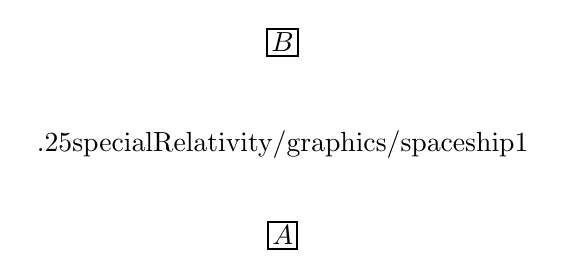
\begin{tikzpicture}
    \node at (0,0) {\pic{.25}{specialRelativity/graphics/spaceship1}};
    \node[thick,draw=black,inner sep=1.5pt] at (0,1.3) {$B$};
    \node[thick,draw=black,inner sep=1.5pt] at (0,-1.15) {$A$};
  \end{tikzpicture}
  \caption{Shining a light from inside a spaceship}
  \label{fig:time-dilation1}
\end{figure}
The light originates from point $A$ reflects off a mirror on the other side of
the ship, at point $B$, and finally returning to point $A$ again. Since the
speed of light $c$ is constant, the time it takes for the light to travel from
$A$ to $B$ is defined as
\begin{equation}
  t=\frac{|AB|}c
\end{equation}
(More precisely, the astronaut would measure a time of $2t$ for the light pulse
to travel twice the distance and return to point $A$.) We will call this time
\textbf{proper time} because $t$ is measured by an observer \emph{at rest}
relative to the events.
%I know the speed of light $c$, and I know how long it took for the light pulse
%to reach $B$. (For convenience, we will use $t$ instead of $\Delta t$ for time
%interval.)

Now, an observer on the planet is also watching the light pulse being fired
on-board the spaceship as well, as shown in Fig.~\ref{fig:time-dilation2}.
\begin{figure}[ht]
  \centering
  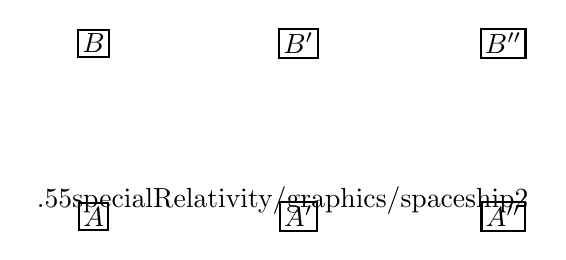
\begin{tikzpicture}
    \node at (0,0) {\pic{.55}{specialRelativity/graphics/spaceship2}};
    \node[thick,draw=black,inner sep=1.5pt] at (-2.4,2) {$B$};
    \node[thick,draw=black,inner sep=1.5pt] at (-2.4,-.2) {$A$};

    \node[thick,draw=black,inner sep=1.5pt] at (.2,2) {$B'$};
    \node[thick,draw=black,inner sep=1.5pt] at (.2,-.2) {$A'$};

    \node[thick,draw=black,inner sep=1.5pt] at (2.8,2) {$B''$};
    \node[thick,draw=black,inner sep=1.5pt] at (2.8,-.2) {$A''$};
  \end{tikzpicture}
  \caption{Watching a beam of laser from outside a spaceship}
  \label{fig:time-dilation2}
\end{figure}
The observer on the planet is also in an inertial frame of reference: as far as
she is concerned, she is stationary, and the spaceship and the astronaut inside
are moving with constant velocity. But her observation of the laser beam is
different: the same light pulse will originate from point $A$, but will reflect
off the mirror at $B'$, and finally returning to the bottom of the ship at
point $A''$. It is clear that, from the planet's frame of reference, the light
has to travel a longer distance from $A\rightarrow B\rightarrow B''$ than from
$A\rightarrow B\rightarrow A$. As the speed of light is also $c$ from her
frame of reference, therefore the time it takes for the light pulse to travel
from $A$ to $B'$,
\begin{equation}
  t'=\frac{|AB'|}c
\end{equation}
is longer than $t$ (i.e. $t'>t$). (Again, the measurement of time would be
taken for the light to travel from $A$ to $B'$ and back to $A''$, and then
divided by 2.) We will call $t'$ the \textbf{dilated time} because it is
measured by an observer in another inertial frame that is \emph{moving}
relative to the events. 

We can relate the proper time $t$ and dilated time $t'$ by the velocity $v$ of
the ship, and with a straight forward application of Pythagorean theorem, as
shown in Fig.~\ref{fig:time-dilation3}.
\begin{figure}[ht]
  \centering
  \begin{tikzpicture}[vectors,red]
    \draw (0,0)--(0,2)
    node[pos=0,below left,black]{$A$} node[midway,left,black]{$ct$}
    node[left,black] {$B$};
    \draw (0,2)--(4,2) node[midway,above,black]{$vt'$} node[right,black]{$B'$};
    \draw (0,0)--(4,2) node[midway,below, black]{$ct'$};
  \end{tikzpicture}
  \caption{Relating proper time and dilated time}
  \label{fig:time-dilation3}
\end{figure}
Relating the velocity $v$ of the spaceship, speed of light $c$ and the observed
times $t$ and $t'$:
\begin{equation*}
  (ct')^2 =(vt')^2 + (ct)^2
\end{equation*}
Grouping the $t'$ terms on the left side:
\begin{equation*}
  \left(c^2-v^2\right)t'^2 =c^2t^2
\end{equation*}
Dividing both sides by $c^2$, and solving for $t'$, we have the same equation
for time dilation:
\begin{equation}
  \boxed{t'=\frac t\bigsqrt}
  \label{eq:time-dilation}
\end{equation}
Since the $\bigsqrt$ is always less than 1, dilated time $t'$ is always longer
than proper time $t$, in other words,
\begin{definition}
  \textbf{Relativity of time:} a running clock runs slow.
\end{definition}
We define the \textbf{Lorentz factor} $\gamma$ as a short-hand for writing
the factor for time dilation (and later, for length contraction, relativistic
momentum and mass):
\begin{equation}
  \boxed{\gamma=\lorentz}
\end{equation}
So the Eq.~\ref{eq:time-dilation} can be written as:
\begin{equation}
  \boxed{
    t' =\gamma t
  }
\end{equation}

We can best explain how time dilation works in the next two examples:
%We can relate the time interval observed by me on the spaceship ($t$) and
%your time interval on the small planet ($t'$) using Pythagorean theorem:
%  
%\textbf{Relativity of time}: the passage of time as measured by
%two observers in two different inertial references are different
%
%
%
%
%\section{Relativity of Time: Time Dilation}
%The passage of time as measured by two observers in two different inertial
%frames of reference are related by:
%\begin{equation}
%  \boxed{t'=\frac t\bigsqrt}
%\end{equation}
%\begin{center}
%  \begin{tabular}{l|c|c}
%    \rowcolor{pink}
%    \textbf{Variable} & \textbf{Symbol} & \textbf{SI Unit}\\ \hline
%    Proper time (ordinary time)  & $t$  & \si\second \\
%    Dilated time (expanded time) & $t'$ & \si\second \\
%    Speed               & $v$ & \si{\metre\per\second}\\
%    Speed of light      & $c$ & \si{\metre\per\second}
%  \end{tabular}
%\end{center}
%\begin{itemize}    
%\item\textbf{Proper time}
%\item
%\end{itemize}
%
%
%
%
%%\section{Relativity of Time: Time Dilation}
%%  Since $\bigsqrt<1$, $t'>t$.
%%
%
%
%
\begin{example}\index{time dilation!example}
  \label{example:time1}
  Kim is riding a rocket that speeds past an asteroid at $v=0.800c$ (i.e.\
  \SI{80.0}{\percent} of the speed of light. If Kim sees \SI{10.0}{\second}
  pass on her watch, how long would that time interval be as seen by Jim, an
  observer on the asteroid?
  
  \textbf{Solution:}
  \begin{itemize}[leftmargin=15pt]
  \item Kim is stationary relative to the watch. As far as Kim is concerned,
    she, her watch, and the rocket are all stationary, therefore the time that
    she measures (\SI{10.0}\second) is the \emph{proper time}.
  \item Jim see's Kim's watch moving, therefore Jim is in a moving reference
    frame, and he measures the \emph{dilated time}:
    \begin{displaymath}
      t' =\frac t\bigsqrt=\frac{10.0}{\sqrt{1-0.800^2}}=\SI{16.7}\second
    \end{displaymath}
  \end{itemize}
  In the time it took Kim's watch to run \SI{10.0}\second, Jim's watch has gone
  \SI{16.7}\second, therefore Jim concludes that Kim's watch (which is moving
  relative to him) is running slow. Our conclusion from this example is that
  \textbf{a moving clock appears to run slow}.
\end{example}
But let's try the same example in reverse.
\begin{example}\index{time dilation!example}
  Kim is riding a rocket that speeds past an asteroid at $0.800c$. If Jim, an
  observer in the \emph{asteroid}, sees \SI{10.0}{\second} pass on his watch,
  how long would that time interval be as seen by Kim?
  \begin{itemize}
  \item Jim is stationary relative to his watch. As far as Jim is concerned,
    he, his watch, and the asteroid are all stationary, therefore he measures
    the \emph{proper time}.
  \item Kim see's Jim's watch moving, therefore Kim is in a moving reference
    frame, and she measures the \emph{dilated time}:
    \begin{displaymath}
      t' =\frac t\bigsqrt=\frac{10.0}{\sqrt{1-0.800^2}}=\SI{16.7}\second
    \end{displaymath}
  \item This problem is exactly the same as the last one!
  \item Kim observes that in the time it took Jim's clock to run
    \SI{10.0}\second, her watch has already gone \SI{16.7}\second, therefore
  \item Kim concludes that Jim's watch must be running slow
  \end{itemize}
\end{example}

How can the observer on the asteroid think that the rocket's clock is running
slow, while the observer on the rocket thinks that the asteroid's clock is
the one running slow? The answer lies with the relativity of simultaneity. The
watches on the asteroid and on the rocket are \emph{not} synchronized.

In Example \ref{example:time1}, when Kim (on the rocket) starts measuring a
\SI{10.0}{\second} time interval, in order for Jim to compare that interval to
\emph{his} watch, he has to start and end at the same time (simultaneously!) as
Kim. And we will assume that he was successful in doing just that\ldots in his
own frame of reference. But simultaneity is relative: in Kim's reference frame,
Jim never got the timing right! This problem reverses when Kim also
\emph{tries} to synchronize her watch to Jim's \SI{10.0}{\second} interval.


\section{Relativity of Space: Length Contraction}\index{length contraction}
Captain Quick is a comic book hero who can run at nearly the speed of light.
In his hand, he is carrying a bomb with a lit fuse set to explode in
\SI{1.50}{\micro\second}. The bomb must be placed into its bracket before
this happens. The distance ($L$) between the bomb and the bracket is
\SI{402}\metre.
%
%
%
%
%\section{Relativity of Space: Length Contraction}
\begin{figure}[ht]
  \centering
  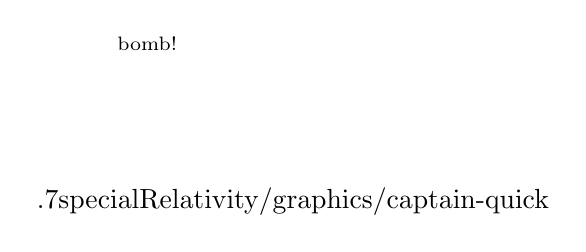
\begin{tikzpicture}
    \node at (0,0) {\pic{.7}{specialRelativity/graphics/captain-quick}};
    \node[fill=white] at (-1.85,2) {\scriptsize bomb!};
  \end{tikzpicture}
\end{figure}
Both Captain Quick and the observers on the side of the road agree that
he is moving at $v=\SI{2.00e8}{\metre\per\second}$ relative to the bracket.
%
%
%
%
%\section{Relativity of Space: Length Contraction}
If Captain Quick runs at \SI{2.00e8}{\metre\per\second}, according to
classical mechanics, he does not make it in time:
\begin{displaymath}
  t'=\frac Lv=\frac{402}{\num{2.00e8}}
  =\SI{2.01e-6}\second=\SI{2.01}{\micro\second}
\end{displaymath}
In fact, this \emph{is} the amount of time that the observer on the side of
the road measures. However, the bomb will \emph{not} explode.




%\section{Relativity of Space: Length Contraction}
To the observer at the side of the road, time on the bomb is slowed due to
time dilation. A time interval of $t'=\SI{2.01}{\micro\second}$ observed on
the side of the road is, according to Captain Quick:
\begin{displaymath}
  t' = \frac t\bigsqrt\quad\longrightarrow\quad
  t = t'\bigsqrt
  = 2.01\sqrt{1-\left(\frac{2.00}{3.00}\right)^2}
  = \boxed{\SI{1.50}{\micro\second}}
\end{displaymath}
The observer on the side of the road sees a passage of (dilated) time of
$t'=\SI{2.01}{\micro\second}$, but Captain Quick, who is stationary relative
to the bomb, experiences a passage of (proper) time of only
$t=\SI{1.50}{\micro\second}$, just in time to put the bomb into the bracket
before it explodes.
%
%
%
%
%\section{Relativity of Space: Length Contraction}
If Captain Quick sees only $t=\SI{1.50}{\micro\second}$, then how \emph{far}
did he travel? From his frame of reference, the bracket is moving towards him
at $v=\SI{2.00e8}{\metre\per\second}$. In this time, the bracket travels:
\begin{displaymath}
  L'=vt=\boxed{\SI{300}\metre}
\end{displaymath}
%  
%  \textbf{A moving object is contracted in length along the direction of
%    motion.}
%
%
%
%
%
%\section{Relativity of Space: Length Contraction}
An stationary observer sees the length of an object moving at speed $v$
contracted by the same factor as time dilation:  
\begin{equation}
  \boxed{L'=L\bigsqrt}
\end{equation}
\begin{center}
  \begin{tabular}{l|c|c}
    \rowcolor{pink}
    \textbf{Variable} & \textbf{Symbol} & \textbf{SI Unit}\\ \hline
    Proper length     & $L$  & \si\second \\
    Contracted length & $L'$ & \si\second \\
    Speed             & $v$ & \si{\metre\per\second}\\
    Speed of light    & $c$ & \si{\metre\per\second}
  \end{tabular}
\end{center}

Length contraction only occurs in the direction of motion.
Fig.~\ref{fig:baseball} shows how a baseball will appear to a moving observer
as it approaches near the speed of light. However, if you are a small insect
sitting on the baseball, you will not observe any length contraction.

\begin{figure}[ht]
  \centering
  \begin{minipage}{1.5in}
    \centering
    \includegraphics[width=1.3in]{specialRelativity/baseball}\\
    $v=0$
  \end{minipage}
  \hspace{\stretch1}
  \begin{minipage}{1in}
    \centering
    \includegraphics[height=1.3in,width=1.12in]{specialRelativity/baseball}\\
    $v=0.5c$
  \end{minipage}
  \hspace{\stretch1}
  \begin{minipage}{1in}
    \centering
    \includegraphics[height=1.3in,width=.567in]{specialRelativity/baseball}\\
    $v=0.9c$
  \end{minipage}
  \begin{minipage}{1in}
    \centering
    \includegraphics[height=1.3in,width=.183in]{specialRelativity/baseball}\\
    $v=0.99c$
  \end{minipage}
  \begin{minipage}{1in}
    \centering
    \includegraphics[height=1.3in,width=0.06in]{specialRelativity/baseball}\\
    $v=0.999c$
  \end{minipage}
  \caption{Length contraction of a baseball if it can travel near the speed of
    light}
  \label{fig:baseball}
\end{figure}


\begin{example}
  A spacecraft passes Earth at a speed of \SI{2.00e8}{\metre\per\second}. If
  observers on Earth measure the length of the spacecraft to be \SI{554}\metre,
  how long would it be according to its passengers?
\end{example}


%\section{Lorentz Factor}

%  Then time dilation and length contraction can be written simply as:
%
%  \eq{-.1in}{
%    \boxed{t' = \gamma t}\quad\quad\boxed{L' = \frac L\gamma}
%  }
%
%
%
%

%
%
%
%
%\section{Let's Summarize}
%\begin{center}
%  \begin{tikzpicture}[scale=2,vectors]
%    \draw (1,.5)--(2,.5) node[pos=0,left] {\textbf{A}};
%    \draw (3,0)--(2,0) node[pos=0,right]{\textbf{B}};
%  \end{tikzpicture}
%\end{center}
%If A and B are moving uniformly with respect to one another (doesn't matter
%if they're moving towards, or away from each other)
%\begin{itemize}
%\item They do not agree whether any events happens at the same time or not
%\item Each sees the other's clock running slow
%\item Each sees the other ``contracted'' in length along the direction of
%  motion
%\end{itemize}



%\section{Lorentz Transformation}
%  Time dilation and length contraction only tell part of the story. To account
%  for the loss of simultaneity from one inertial frame to another, we need to
%  use the \textbf{Lorentz transformation:}
%
%  \vspace{-.3in}{\large
%    \begin{align*}
%      x' &= \gamma(x-vt)\\
%      y' &= y\\
%      z' &= z\\
%      t' &=\gamma\left(t-\frac{vx}{c^2}\right)
%    \end{align*}
%  }
%  
%  The Lorentz transformation ``solves'' many paradoxes (e.g.\ the twin paradox)
%  from the time-dilation and length-contraction equations, but aren't really
%  there.
%
%  For slow speeds $v\ll c$, Lorentz transformation reduces to the Galilean
%  transformation from classical mechanics, from which the velocity addition
%  rule is formulated:
%
%  \vspace{-.3in}{\large
%    \begin{align*}
%      x' &= x-vt\\
%      y' &= y\\
%      z' &= z\\
%      t' &= t'
%    \end{align*}
%  }
%
%
%
\section{Relative Motion}

The Galilean velocity addition rule violates the postulates of relativity,
so Einstein replaces it with \textbf{Einstein velocity addition rule}:
\begin{equation}  
  \boxed{v_{AC}=\frac{v_{AB}+v_{BC}}{1+\dfrac{v_{AB}v_{BC}}{c^2}}}
\end{equation}
When velocities are slow compared to the speed of light ($v_{AB}\ll c$, and
$v_{BC}\ll c$) we recover the Galilean velocity addition rule.


%%\section{But What About\ldots}
%%  We have studied the most important principles in special relativity already,
%%  but what about:
%%
%%  \vspace{-.2in}{\Huge
%%    \begin{displaymath}
%%      \boxed{E=mc^2}
%%    \end{displaymath}
%%  }
%%
%%  We seem to be no closer to learning about it!
%%
%
%
%
\section{Relativistic Momentum}
Recall that momentum is mass times velocity (displacement over time). But
since $\Delta\vec x$ and $t$ both depend on the motion, we need modify
the expression for \emph{relativistic} motion:
\begin{equation} 
    \boxed{
      p
      %=m\frac{\Delta\vec x}t
      %=\frac{m\Delta\vec x}{t'\bigsqrt}
      %=\frac{m\vec v}\bigsqrt
      =\gamma mv
    }
\end{equation}
%\begin{center}
%  \begin{tabular}{l|c|c}
%    \rowcolor{pink}
%    \textbf{Variable} & \textbf{Symbol} & \textbf{SI Unit}\\ \hline
%    Relativistic momentum & $p$ & \si{\kilo\gram}\\
%    (Rest) mass & $m$ & \si{\kilo\gram}\\
%    Speed & $v$ & \si{\metre\per\second}\\
%    Lorentz Factor & $\gamma$ & (no unit)
%  \end{tabular}
%\end{center}
We have not changed the \emph{definition} of momentum, only the underlying
assumptions about space and time when calculating momentum.




\section{Relativistic Mass}
Relativistic momentum shows that mass is also relativistic: The
\textbf{apparent mass}\footnote{also known as \textbf{relativistic mass}} $m'$
as measured by a moving observer is related to its
\textbf{rest mass}\footnote{also known as \textbf{intrinsic mass} or
\textbf{invariant mass}} $m$ are related by:
\begin{equation}
  \boxed{m'=\frac m\bigsqrt=
    \gamma m}
\end{equation}
%\begin{center}
%  \begin{tabular}{l|c|c}
%    \rowcolor{pink}
%    \textbf{Variable} & \textbf{Symbol} & \textbf{SI Unit}\\ \hline
%    Relativistic mass (measured in moving frame) & $m'$ & \si{\kilo\gram}\\
%    Rest mass (measured in stationary frame) & $m$  & \si{\kilo\gram}\\
%    %Speed               & $v$ & \si{\metre\per\second}\\
%    %Speed of light      & $c$ & \si{\metre\per\second}
%      Lorentz Factor      & $\gamma$ & (no unit)
%  \end{tabular}
%\end{center}
As an object speeds up, it behaves as if it is more massive. As
$v\rightarrow c$, $m'\rightarrow\infty$.




\begin{example}
  An electron has a rest mass of \SI{9.11e-31}{\kilo\gram}. In a detector, it
  behaves as if it has a mass of \SI{12.55e-31}{\kilo\gram}. How fast is that
  electron moving relative to the detector?
\end{example}


\section{Mass-Energy Equivalence}

%\section{Work and Energy}
Einstein published a fourth paper in \emph{Annalen der Physik} on November
21, 1905 (received Sept.\ 27) titled ``Does the Inertia of a Body Depend Upon
Its Energy Content?''\footnote{In German: Ist die Tr\"{a}gheit eines
K\"{o}rpers von seinem Energieinhalt abh\"{a}ngig?}. In this paper, Einstein
deduced the most famous of equations: $E=mc^2$

%\section{Work and Energy}
Net force is the rate of change of momentum with respect to time. \emph{This
definition has not changed.}

%  \eq{-.1in}{
%    \vec F=\diff{\vec p}t
%  }

Work is the integral of the dot product between force and displacement
vectors. \emph{This definition has not changed.}

%  \eq{-.1in}{
%    W=\int\vec F\cdot\dl\vec x=\int\diff{\vec p}t\cdot\dl\vec x
%  }

Since we now have a relativistic expression for momentum, we substitute that
new expression into the expression for force, and then integrate.




\subsection{Mechanical Work}
For 1D motion\footnote{Because math is hard, and solving this problem in
higher dimensions isn't any more insightful than 1D.}, we can rearrange the
terms in the integral:

%  \eq{-.12in}{
%    W=\int F\dl x=\int\diff pt\dl x=\int v\dl p
%  }
%  
Since both $v$ and $p$ are continuous in time, we can apply the chain rule to
find the infinitesimal change in momentum ($\dl p$) with respect to $\gamma$
and $v$:
  
%  \eq{-.15in}{
%    p=\gamma mv \quad\longrightarrow\quad\dl p= \gamma\dl v +v\dl\gamma
%  }

Substituting that back into the integral, we have:
  
%  \eq{-.1in}{
%    W=\int v\dl p=\int mv(\gamma\dl v +v\dl\gamma)=
%    \int m\left(\gamma v\dl v +v^2\dl\gamma\right)
%  }




One of the integral is with respect to $\gamma$, so we express $v$ and $\dl v$
in terms of $\gamma$ using the definition of Lorentz transformation:

%  \eq{-.1in}{
%    v^2=c^2\left[1-\left(\frac1\gamma\right)^2\right]
%    \quad\longrightarrow\quad
%    \dl v=\frac{c^2}{\gamma^3v}\dl\gamma
%  }

Putting everything together, we have a surprisingly simple integral:

%  \eq{-.15in}{
%    W=\int m(\gamma v\dl v +v^2\dl\gamma)=\int m\left[\frac{c^2}{\gamma^2}+
%      c^2\left(1-\frac1{\gamma^2}\right)\right]\dl\gamma
%    = \int_1^\gamma mc^2\dl\gamma
%  }

The limit of the integral is from 1 because at $v=0$, $\gamma=1$




\subsection{Work-Energy Theorem}
The integral is reasonably simple:

%  \eq{-.12in}{
%    W=\int_1^\gamma mc^2\dl\gamma=\gamma mc^2-mc^2
%  }
%  
From the work-energy theorem, this expression is equal to the change in kinetic
energy. And since the integral is computed from $v=0$, this is just the
\textbf{relativistic kinetic energy}:
  
%  \eq{-.15in}{
%    \boxed{K=\gamma mc^2-mc^2}
%  }
%\begin{center}
%  \begin{tabular}{l|c|c}
%    \rowcolor{pink}
%    \textbf{Variable} & \textbf{Symbol} & \textbf{SI Unit}\\ \hline
%    Kinetic energy & $K$ & \si\joule \\
%    Rest mass      & $m$ & \si{\kilo\gram} \\
%    Speed of light & $c$ & \si{\metre\per\second} \\
%    Lorentz factor & $\gamma$ & (no units)
%  \end{tabular}
%\end{center}



\section{Relativistic Energy}
%  
%  \eq{0in}{
%    \boxed{K=m'c^2-mc^2}
%  }
%
%  The minimum amount of energy that any object has, regardless of it's motion
%  (or lack of) is its \textbf{rest energy}:
%  
%  \eq{-.2in}{ E_0=mc^2 }
%
%  \vspace{-.2in}The \textbf{total energy} of an object has is
%    
%  \eq{-.15in}{
%    E_T=m'c^2=\gamma mc^2
%  }
%
%  \vspace{-.1in}The difference between total energy and rest energy is the
%  kinetic energy:
%
%  \eq{-.2in}{
%    K=E_T-E_0=(\gamma-1)c^2
%  }
%
%
%
%
%  
%  \eq{-.1in}{
%    \boxed{E=mc^2}
%  }
%
\textbf{Mass-energy equivalence}:
\begin{itemize}
\item Whenever there is a change of energy, there is also a change of mass
\item ``Conservation of mass'' and ``conservation of energy'' must be
  combined into a single concept of \textbf{conservation of mass-energy}
\item Mass-energy equivalence doesn't merely mean that mass can be converted
  into energy, and vice versa (although this is true), but rather, one can be
  converted into the other
  \emph{because they are fundamentally the same thing}
\end{itemize}
%
%
%
%
%%\section{Mass-Energy Equivalence}
%% 
%%  \eq{0in}{
%%    \boxed{E=mc^2}
%%  }
%%  \begin{itemize}
%%  \item\vspace{-.2in}Whenever there is a change of energy, there is also a
%%    change of mass
%%  \item Concepts in classical physics:
%%    \begin{itemize}
%%    \item Conservation of mass
%%    \item Conservation of energy
%%    \end{itemize}
%%    must be combined into a single concept of \textbf{conservation of
%%      mass-energy}
%%  \item Mass-energy equivalence doesn't just mean that mass can be converted
%%    into energy and vice versa (although this is true), but rather, one can be
%%    converted into the other \emph{because they are fundamentally equivalent}
%%  \end{itemize}
%%
%
%
%
\section{Energy-Momentum Relation}
The \textbf{energy-momentum relation} relates an object's rest (intrinsic)
mass $m$, total energy $E$, and momentum $p$:

%  \eq{-.1in}{
%    \boxed{E^2=p^2c^2+m^2c^4}
%  }
%\begin{center}
%  \begin{tabular}{l|c|c}
%    \rowcolor{pink}
%    \textbf{Quantity} & \textbf{Symbol} & \textbf{SI Unit} \\ \hline
%    Total energy   & $E$ & \si\joule \\
%    Momentum       & $p$ & \si{\kilo\gram\metre\per\second}\\
%    Rest mass      & $m$ & \si{\kilo\gram} \\
%    Speed of light & $c$ & \si{\metre\per\second}
%  \end{tabular}
%\end{center}
This equation is derived by squaring the expression for relativistic momentum:
\begin{equation*}
  p=m'v=(\gamma m)v
  \quad\rightarrow\quad
  p^2=\gamma^2m^2v^2=\frac{m^2v^2}{1-\left(\dfrac vc\right)^2}
\end{equation*}
Now we can solve for $v^2$ in terms of $m$, $c$ and $p$:
\begin{equation*}
  p^2\left[1-\left(\dfrac vc\right)^2\right]=m^2v^2
  \quad\rightarrow\quad
  p^2-\frac{p^2v^2}{c^2}=m^2v^2
  \quad\rightarrow\quad
  p^2c^2-p^2v^2=m^2c^2v^2
\end{equation*}
We arrive at
\begin{equation*}
  p^2c^2=(p^2+m^2c^2)v^2
  \quad\rightarrow\quad
  \frac{p^2}{m^2}=\left[1+\left(\frac p{mc}\right)^2\right]v^2
  \quad\rightarrow\quad
  \frac{p^2}{m^2v^2}=\left[1+\left(\frac p{mc}\right)^2\right]=\gamma^2
\end{equation*}

Solving for $v^2$ and substituting it back into the Lorentz factor $\gamma$,
we obtain an alternative expression for $\gamma$ in terms of momentum and
rest mass:
\begin{equation*}
  \gamma =\sqrt{1+\left(\frac p{mc}\right)^2}
\end{equation*}
Inserting this form of the Lorentz factor into the equation for total energy,
we have the energy-momentum equation
\begin{equation}
  E=m'c^2=\gamma mc^2= \sqrt{1+\left(\frac p{mc}\right)^2}
  \quad\rightarrow\quad
  E^2=m^2c^4 \left(1+\frac{p^2}{m^2c^2}\right)
  =p^2c^2+m^2c^4
\end{equation}
%
%
%
%
%\section{Energy-Momentum Relation}
%  In a rest frame, %(rest frame, centre-of-momentum frame) the
%  momentum is zero, so the equation simplifies to
%
%  \eq{-.1in}{
%    \boxed{ E=mc^2 }
%  }
  
where $m$ is the rest mass of the object. If the object is \textbf{massless},
as is the case for a \textbf{photon}, then the equation reduces to
\begin{equation}
  \boxed{E=pc}\quad\text{(masslass particle)}
\end{equation}







\section{Kinetic Energy: Classical vs.\ Relativistic}
When a physicist ``discovers'' a new physical law, it is not enough that the
new law explains what could not be explained before, but it also has to be
consistent with what is already explained. In the case of kinetic energy, that
means that Einstein's relativistic equation must agree with Newtonian
(classical) mechanics for $v\ll c$. On first glance, the relativistic and
classical expressions for kinetic energy are obviously different:
\begin{center}
  \begin{minipage}{.3\textwidth}
    \centering
    \textbf{Relativistic:}
    \begin{displaymath}
      K=(\gamma-1)mc^2
    \end{displaymath}
  \end{minipage}
  \begin{minipage}{.3\textwidth}
    \centering
    \textbf{Newtonian:}
    \begin{displaymath}
      K=\frac12mv^2
    \end{displaymath}
  \end{minipage}
\end{center}

But are they really that different? If space and time are indeed relative
quantities, then the relativistic equation for $K$ must apply to all velocities.
But we know that when $v\ll c$, the Newtonian expression works perfectly,
i.e.\ The Newtonian expression for $K$ must be a very good approximation for
the relativistic expression for $K$ for $v\ll c$.

We can show the agreement between the relativistic and Newtonian expressions
using the \textbf{binomial series}. For the function $f(x)=(1+x)^\alpha$, the
binomial series expansion is given by:
\begin{equation}  
  (1+x)^\alpha=
  %\sum_{k=0}^\infty\left(
  %\begin{matrix}
  %  \alpha\\
  %  k
  %\end{matrix}
  %\right)
  %x^k=
  1+\alpha x + \frac{\alpha(\alpha-1)}{2!}x^2+\cdots
\end{equation}
In the case of relativistic kinetic energy, we use:
\begin{equation*}
  x=-\left(\frac vc\right)^2\quad\text{\normalsize and}\quad\quad
  \alpha=-\frac12
\end{equation*}
Substituting these terms into the series expansion:
\begin{equation*}
  K
  =({\color{red}\gamma}-1) mc^2
  = \left({\color{red}1+\frac{v^2}{2c^2}+\frac{3v^4}{8c^4}+\cdots}-1
  \right)mc^2
  =\frac{mv^2}2+\frac{3mv^4}{8c^2}+\cdots
\end{equation*}
For $v\ll c$, we can ignore the high-order terms, which reduces the
relativistic kinetic energy equation to the Newtonian equation. This equation
is a quadratic function of speed $v$:
\begin{equation*}
  K\approx\frac12mv^2
\end{equation*}
However, in relativistic mechanics, $K\rightarrow\infty$ as
$v\rightarrow\infty$ with an asymptote at $v=c$, as shown in
Fig.~\ref{fig:kinetic-energy}.
\begin{figure}[ht]
  \centering
  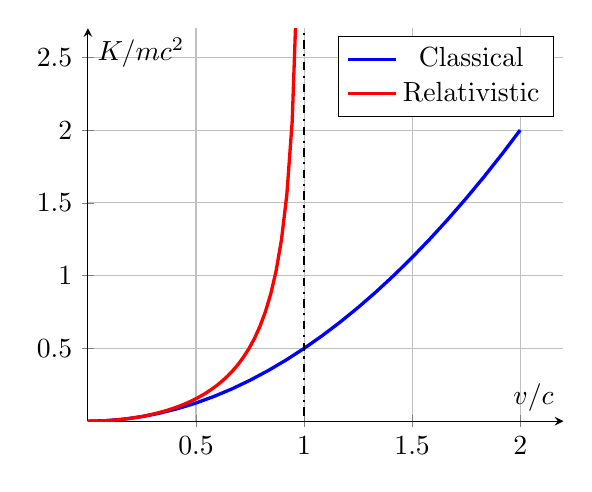
\begin{tikzpicture}
    \begin{axis}[
        axis lines = center,
        grid = both,
        width=3in,
        xmin=0,xmax=2.2, xlabel={$v/c$},
        ymin=0,ymax=2.7, ylabel={$K/mc^2$},
        ytick={0,.5,...,3}
      ]
      \addplot[blue,very thick,domain=0:2]{1/2*x^2};
      \addlegendentry{Classical}
      \addplot[red,very thick,domain=0:.97,samples=40]{1/sqrt(1-x^2)-1};
      \addlegendentry{Relativistic}
      \addplot[thick,dash dot] coordinates{(1,-1)(1,4)};
    \end{axis}
  \end{tikzpicture}
  \caption{Classical and relativistic expressions for kinetic energy diverge
    as speeds approach the speed of light.}
  \label{fig:kinetic-energy}
\end{figure} 
These two equations are in good agreement for $v<0.3c$. Only at higher speeds
does relativistic effects have to be accounted for.



\begin{example}
  A rocket car with a mass of \SI{2.00e3}{\kilo\gram} is accelerated from rest
  to \SI{1.00e8}{\metre\per\second}. Calculate its kinetic energy:
  \begin{enumerate}
  \item Using the classical equation
  \item Using the relativistic equation
  \end{enumerate}
\end{example}
